\chapter{Micro Cathode}

In this chapter, we will explore the algorithm behavior on a considerably more complex test case. However, we will still be able to compute the deterministic solution, which we will use to verify our results. It is meant to show the applicability of our stochastic method, while also showing its practical limits. The test case is largely inspired by the Zero-Dimensional Plasma Kinetics solver \cite{zdplaskin}.

\section{Introduction}

There are several species considered in this model: \ch{e-}, \ch{Ar}, \ch{Ar+}, \ch{Ar^*}, \ch{Ar2+}. Aside from these, we will also consider certain diffusion losses represented as separate species \ch{e(W)}, \ch{Ar^+(W)}, and \ch{Ar2^+(W)}.

It is meant to represent a zero dimensional uniform argon plasma column created by a micro cathode. The specified parameters of the simulation include the pressure (100$\;$Torr~=~13332.2$\;$Pa), room temperature (300$\;$K), cathode gap length (4$\;$cm) and radius (4$\;$cm). The experiment is powered by 1$\;$kV voltage generator with 100$\;$kOhm series resistance.

\section{Reactions and parameters}

In total, we model 13 reactions in the test case. Two of them -- ionization and recombination -- are identical to the two reaction system, the rest of them thus simply extends it. Moreover, we consider argon excitation (with only one metastable state), diffusion losses and (dis)association of diatomic molecules. All the reactions are listed below.

\begin{center}
\begin{gather*}
\text{Reactions in volume:} \\
\ch{e- + Ar ->[ $k_1$ ] e- + e- + Ar+ }, \\
\ch{e- + Ar ->[ $k_2$ ] Ar^* + e-}, \\
\ch{Ar^* + e- ->[ $k_3$ ] Ar + e- }, \\
\ch{e- + Ar^* ->[ $k_4$ ] Ar+ + e- + e- }, \\ \\
\ch{Ar2+ + e- ->[ $k_5$ ] Ar^* + Ar}, \\
\ch{Ar2+ + Ar ->[ $k_6$ ] Ar+ + Ar + Ar}, \\
\ch{Ar^* + Ar^* ->[ $k_7$ ] Ar2+ + e-}, \\
\ch{Ar+ + Ar + e- ->[ $k_8$ ] Ar + Ar}, \\
\ch{Ar^* + Ar + Ar ->[ $k_9$ ] Ar + Ar + Ar}, \\
\ch{Ar+ + Ar + Ar ->[ $k_{10}$ ] Ar2+ + Ar} \\ \\
\text{Ambipolar diffusion losses:} \\
\ch{ Ar+ ->[ $k_{\rm diff}$ ] Ar^+(W)}, \\
\ch{ Ar2+ ->[ $k_{\rm diff}$ ] Ar2^+(W)}, \\
\ch{ e- ->[ $k_{\rm diff}$ ] e(W)}
\end{gather*}
\end{center}

For the simulation, the first four reaction rates $k_1, k_2, k_3, \text{ and } k_4$ are specified by a table as dependent on the current value of the reduced electric field $E/N$.

TODO: Should I include the tables here? Maybe just a few rows?

The reaction rates $k_6, k_7, k_9$ and $k_{10}$ are constant throughout the simulation with 

\begin{flalign*}
    k_6 = 2.53\cdot10^{-42}\;\rm m^3s^{-1}, \\
    k_7 = 6\cdot10^{-16}\;\rm m^3s^{-1}, \\ 
    k_9 = 1.4\cdot10^{-44}\;\rm m^6s^{-1}, \;
    \rm and \\
    k_{10} = 2.25\cdot10^{-43}\;\rm m^6s^{-1}.
\end{flalign*}

As for the remaining reaction rates (including $k_{\rm diff}$), they are computed as a function of the reduced electric field $E/N$. The ratio $E/N$ is in turn computed from a function depending on the current time of the simulation. Moreover, we compute the electron temperature $T_e$ and the mean electron energy $\langle E \rangle$. In a Maxwell–Boltzmann distribution with three degrees of freedom, these two are bound through the equation $\langle E\rangle = \frac32 \, k_{\text{B}} T_e $, where $k_{\text{B}}$ stands for the Boltzmann constant.    

\section{Deterministic solution}

As in the previous test case, we will start by computing the referential numerical deterministic solution. The figure \ref{fig:MicroCathodeImprovedDeterministic} shows the specie concentration evolution in time, while in figure \ref{fig:MicroCathodeImprovedDeterministicLosses} we can see the corresponding diffusion losses. On the right y-axis, there is the value of the reduced electric field $E/N$ governing the reaction rates in the system.

\begin{figure} 
    \centering
    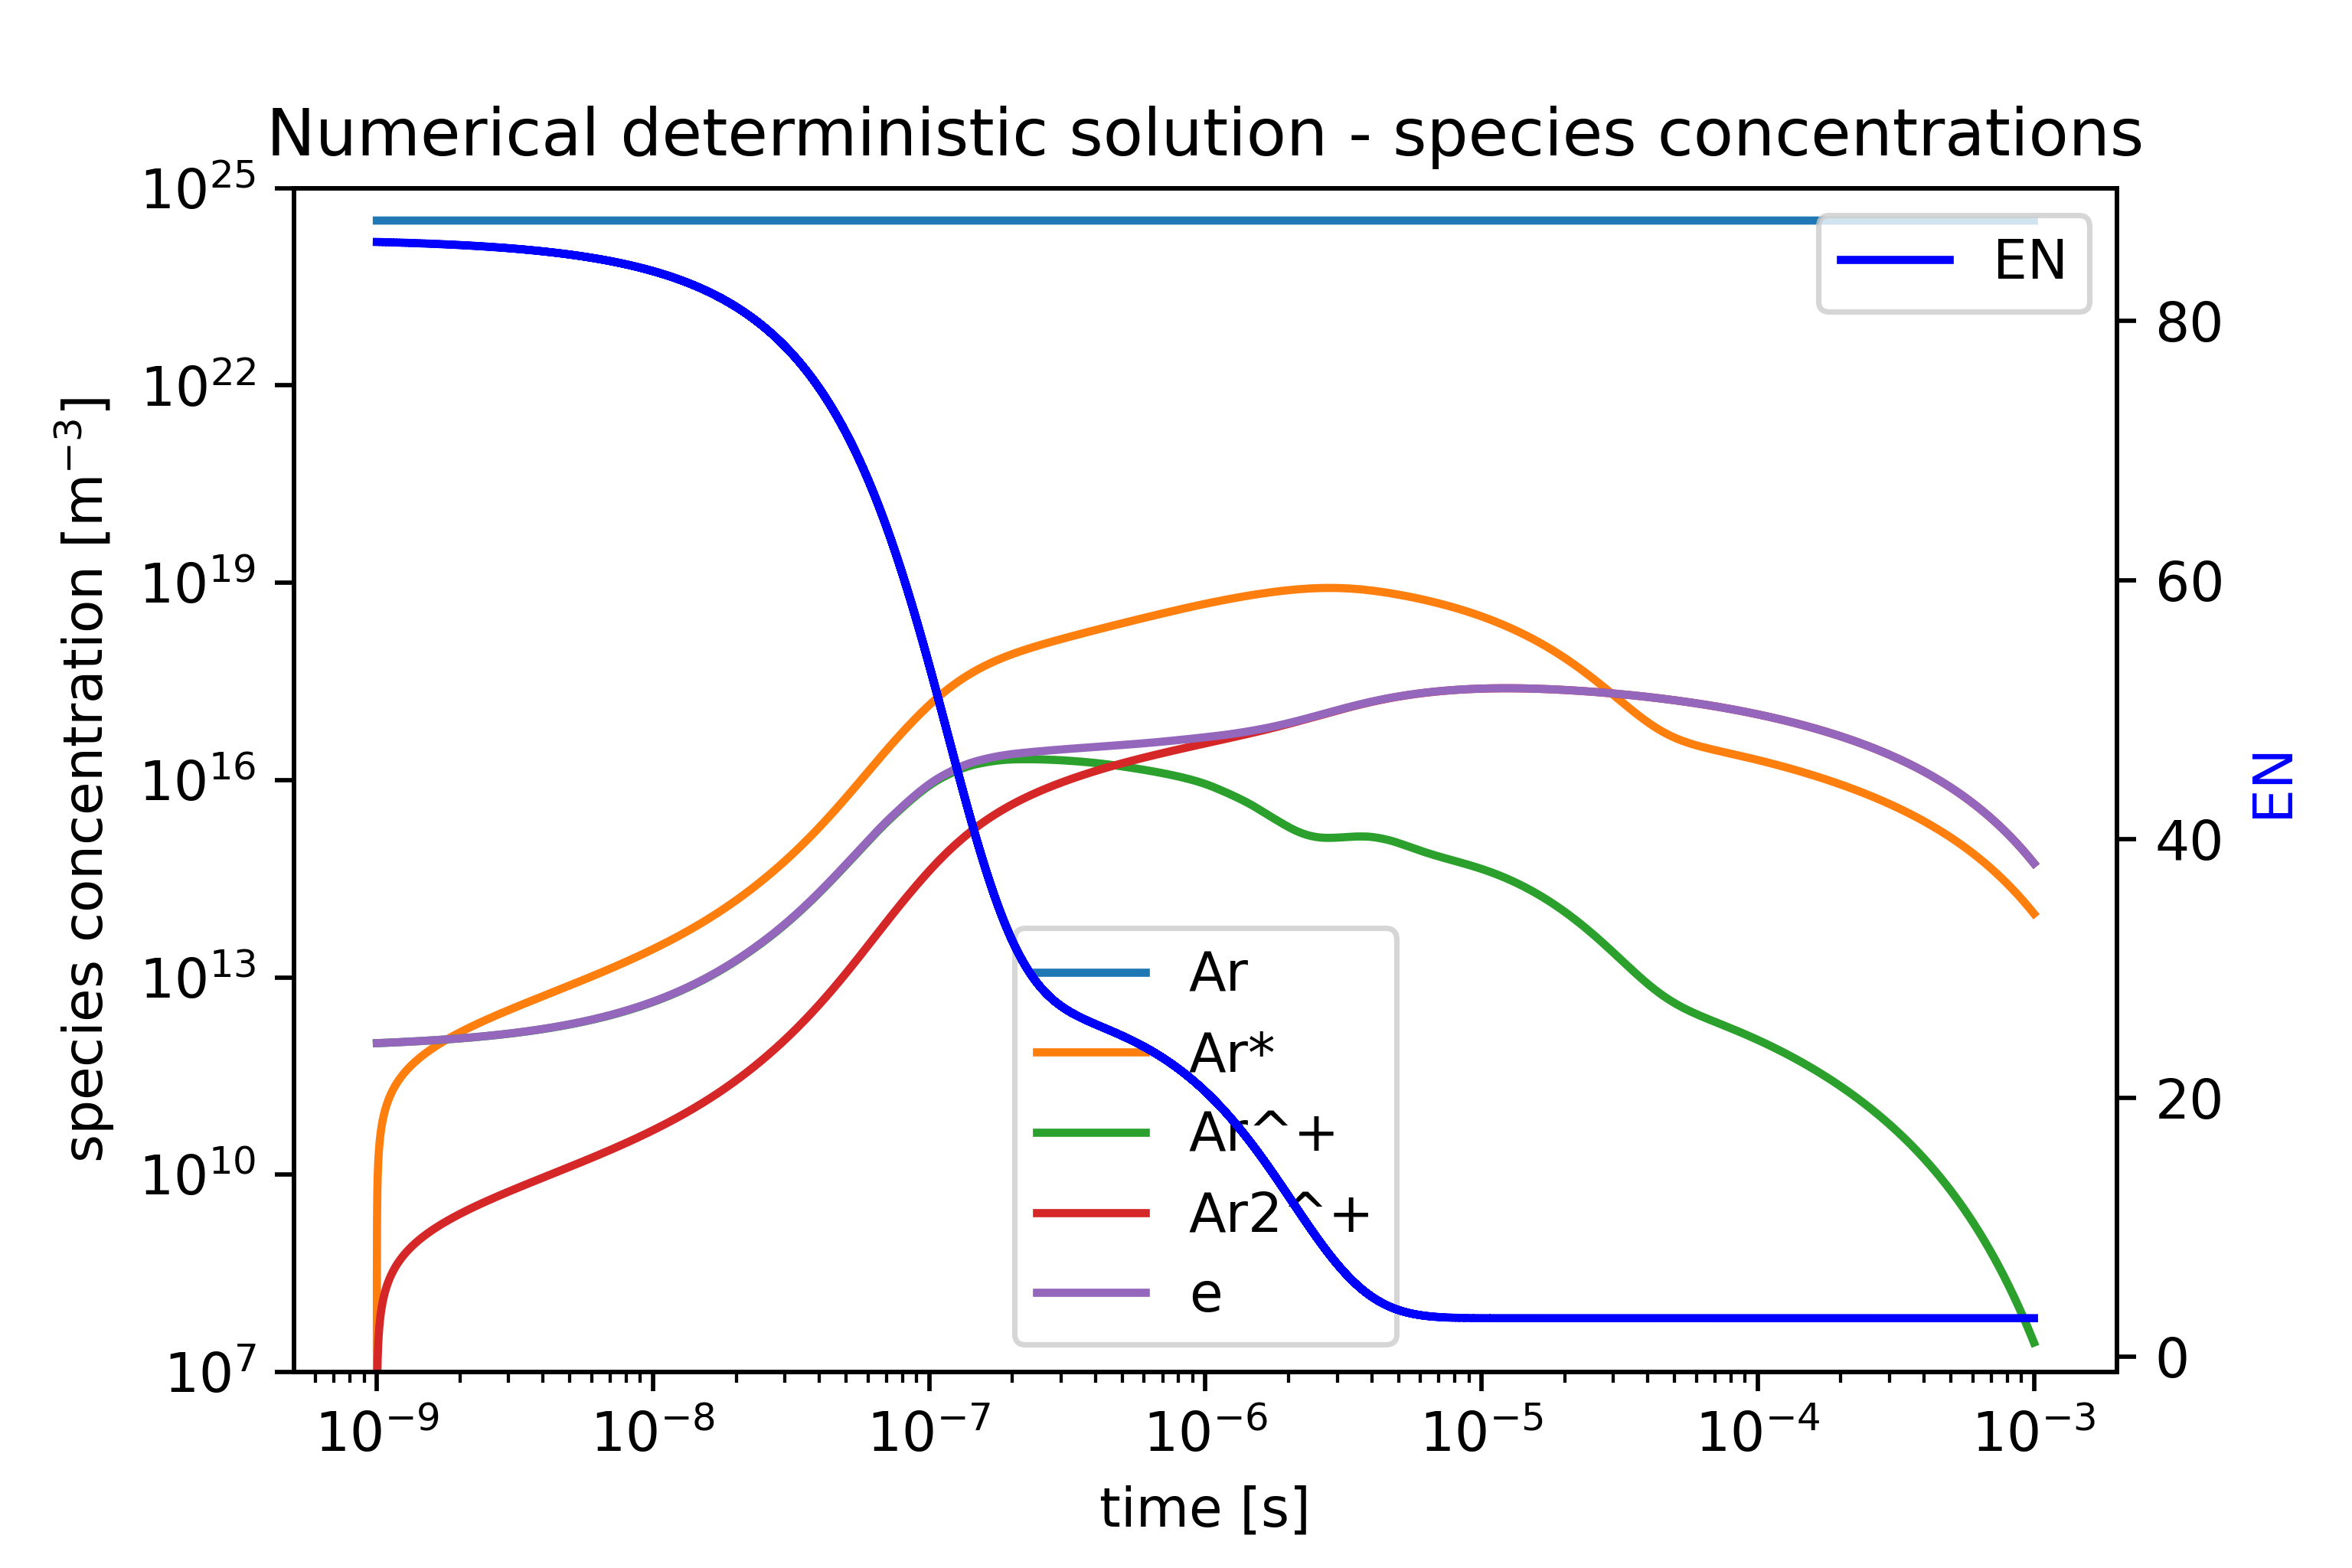
\includegraphics[width=\textwidth]{grafy/MicroCathodeImprovedDeterministic.png}
    \caption{Micro cathode -- numerical deterministic solution for specie concentrations}
    \label{fig:MicroCathodeImprovedDeterministic}
\end{figure}

\begin{figure} 
    \centering
    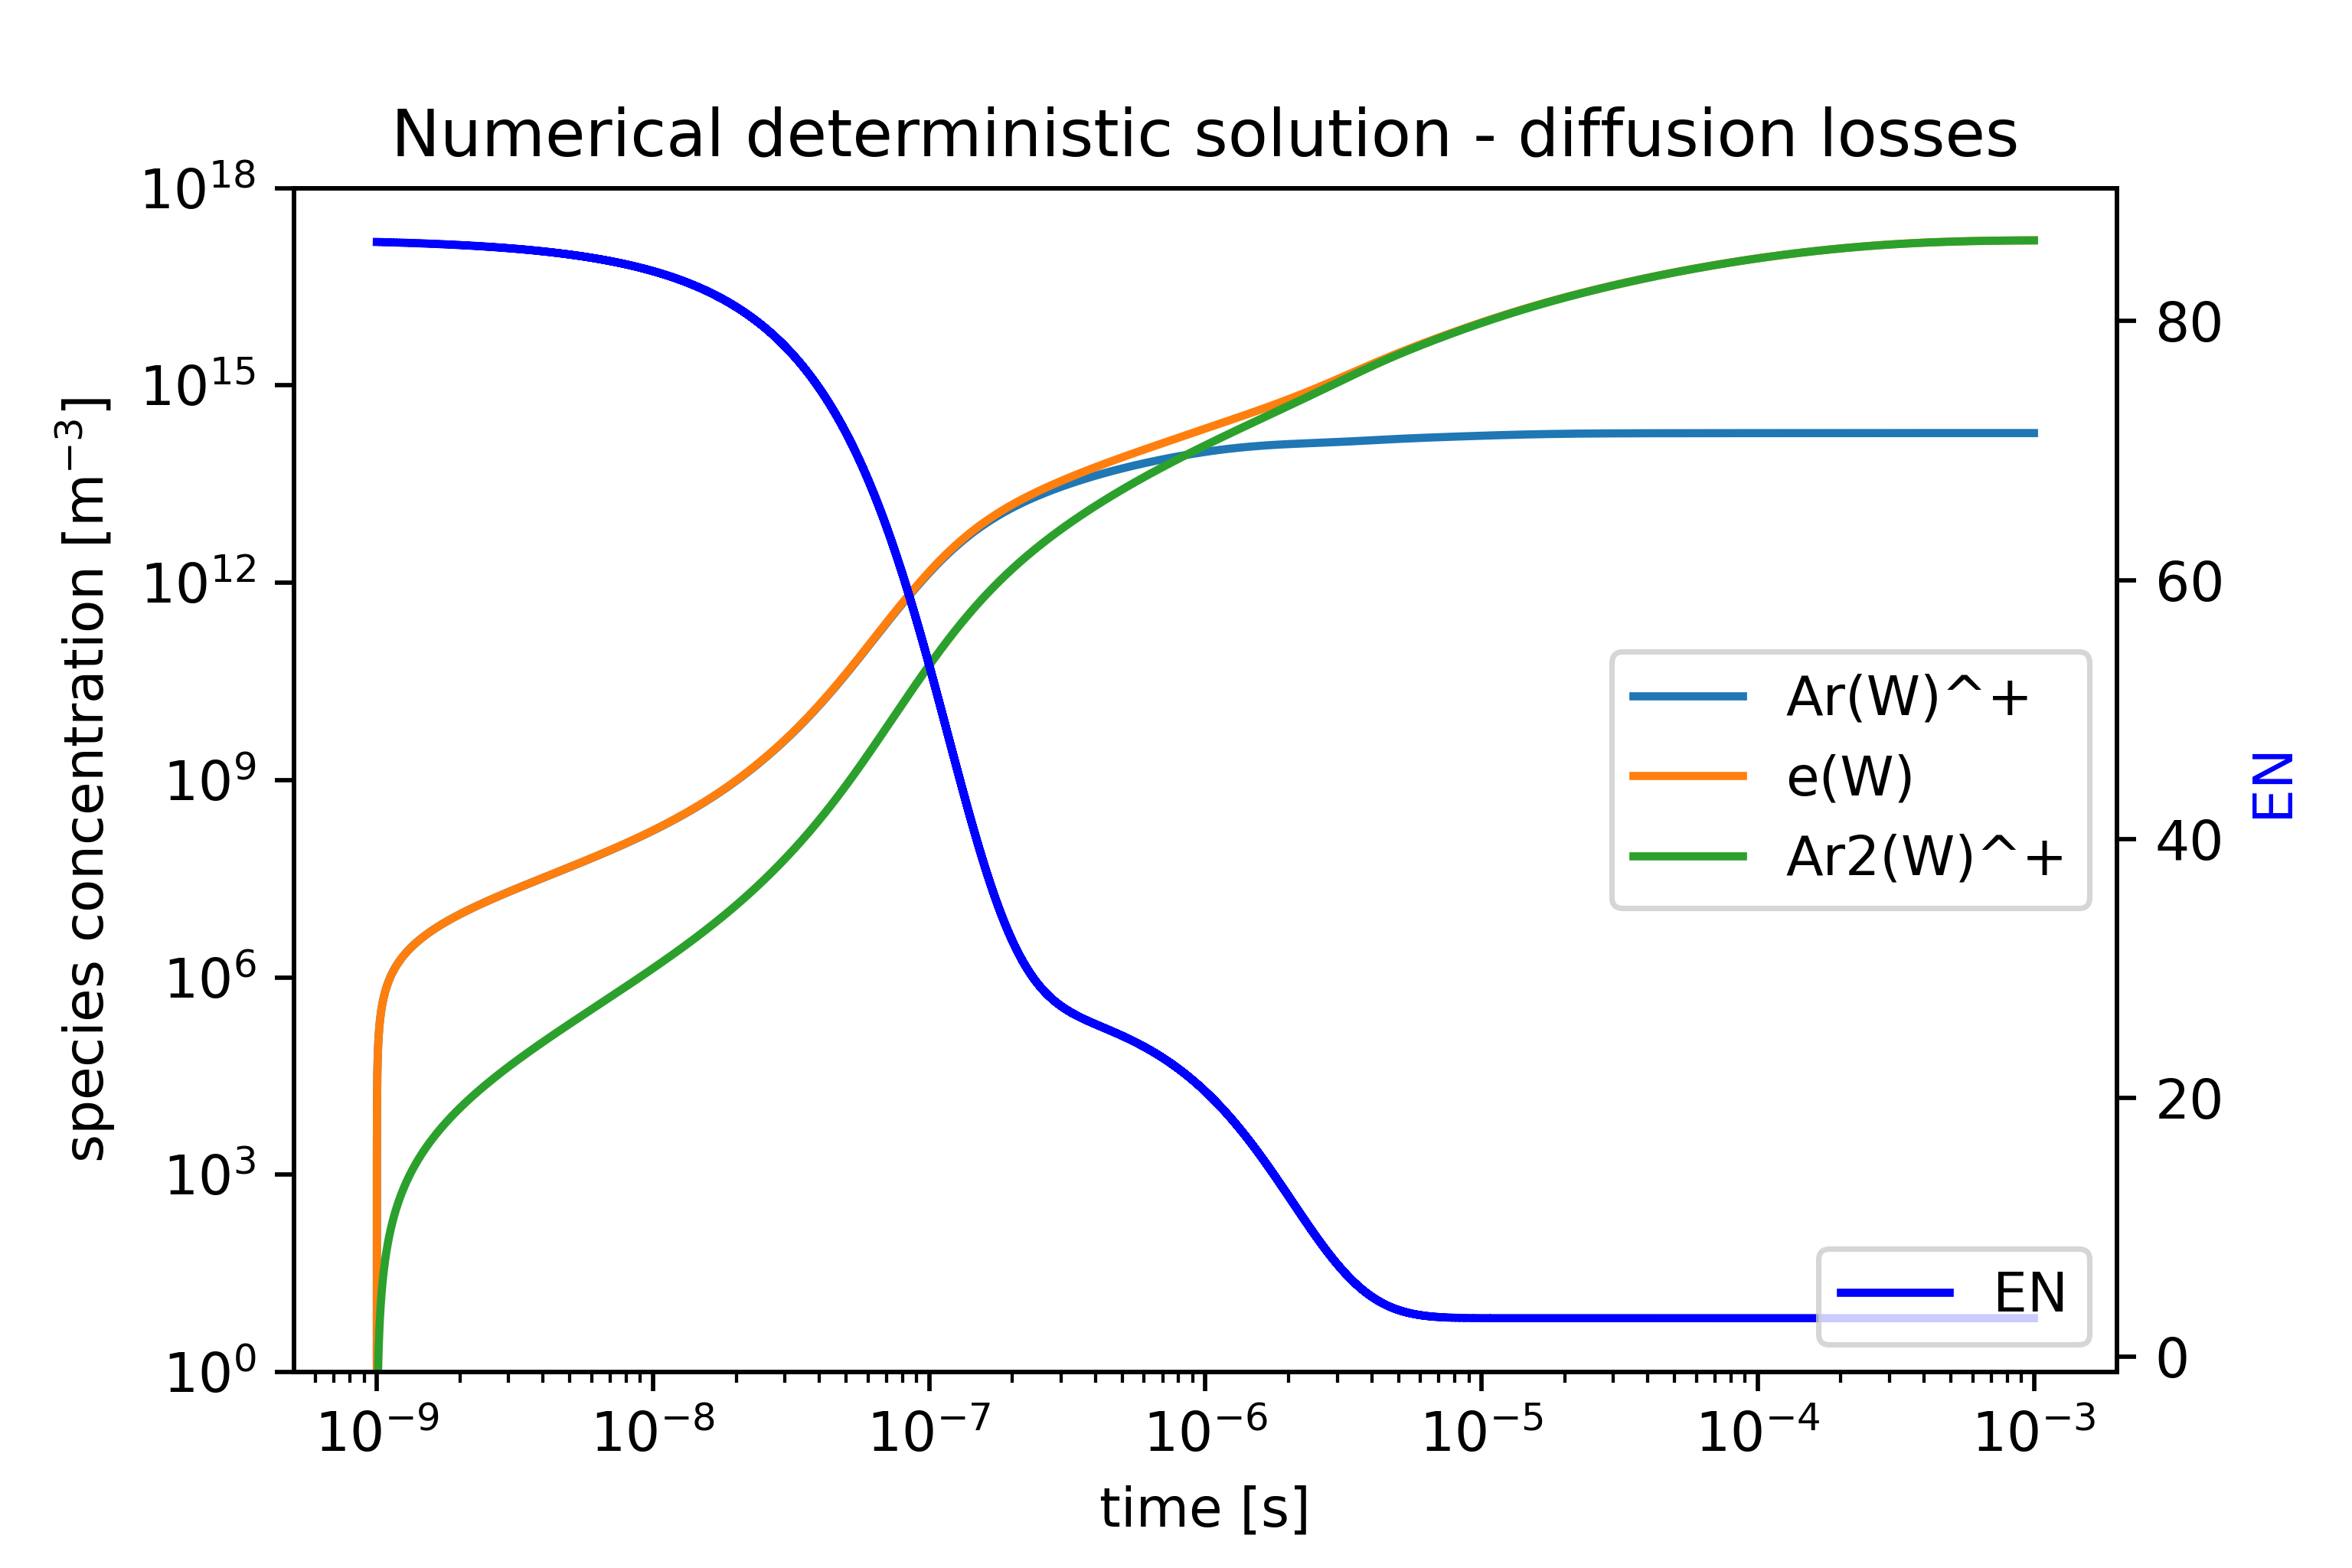
\includegraphics[width=\textwidth]{grafy/MicroCathodeImprovedDeterministicLosses.png}
    \caption{Micro cathode -- numerical deterministic solution for diffusion losses}
    \label{fig:MicroCathodeImprovedDeterministicLosses}
\end{figure}



\section{Monte Carlo solution}

First, we have employed the equal reaction weights method in order to solve this problem. It used exponentially increasing bulk as an extra approximation because otherwise, the system would be too large for any feasible simulation. We do not include the simulation results here, as the figures would completely coincide with those for the deterministic solution. The only visible difference would be when zooming in -- there are barely visible fluctuations in the stochastic solution.

As the equal reaction weights have produced no interesting outputs -- behaving the same as ordinary deterministic solvers, we examine the output of ordinary Monte Carlo solution without the variance reduction technique. Naturally, certain approximation had to be taken -- namely, we use the same exponentially increasing bulk as before. This has led to difficulties towards the end of the simulation. As the \ch{Ar+} concentration decreases, we would need to decrease the bulk value as well in order to model its concentration reliably. However, that would be practically unfeasible as the system is too large and we would almost halt our progress in the simulation time. Therefore, we have reduced the simulation time to roughly half (in absolute value). The evolution of specie concentrations can be seen in figure \ref{fig:MicroCathodeImprovedMC}.

\begin{figure} 
    \centering
    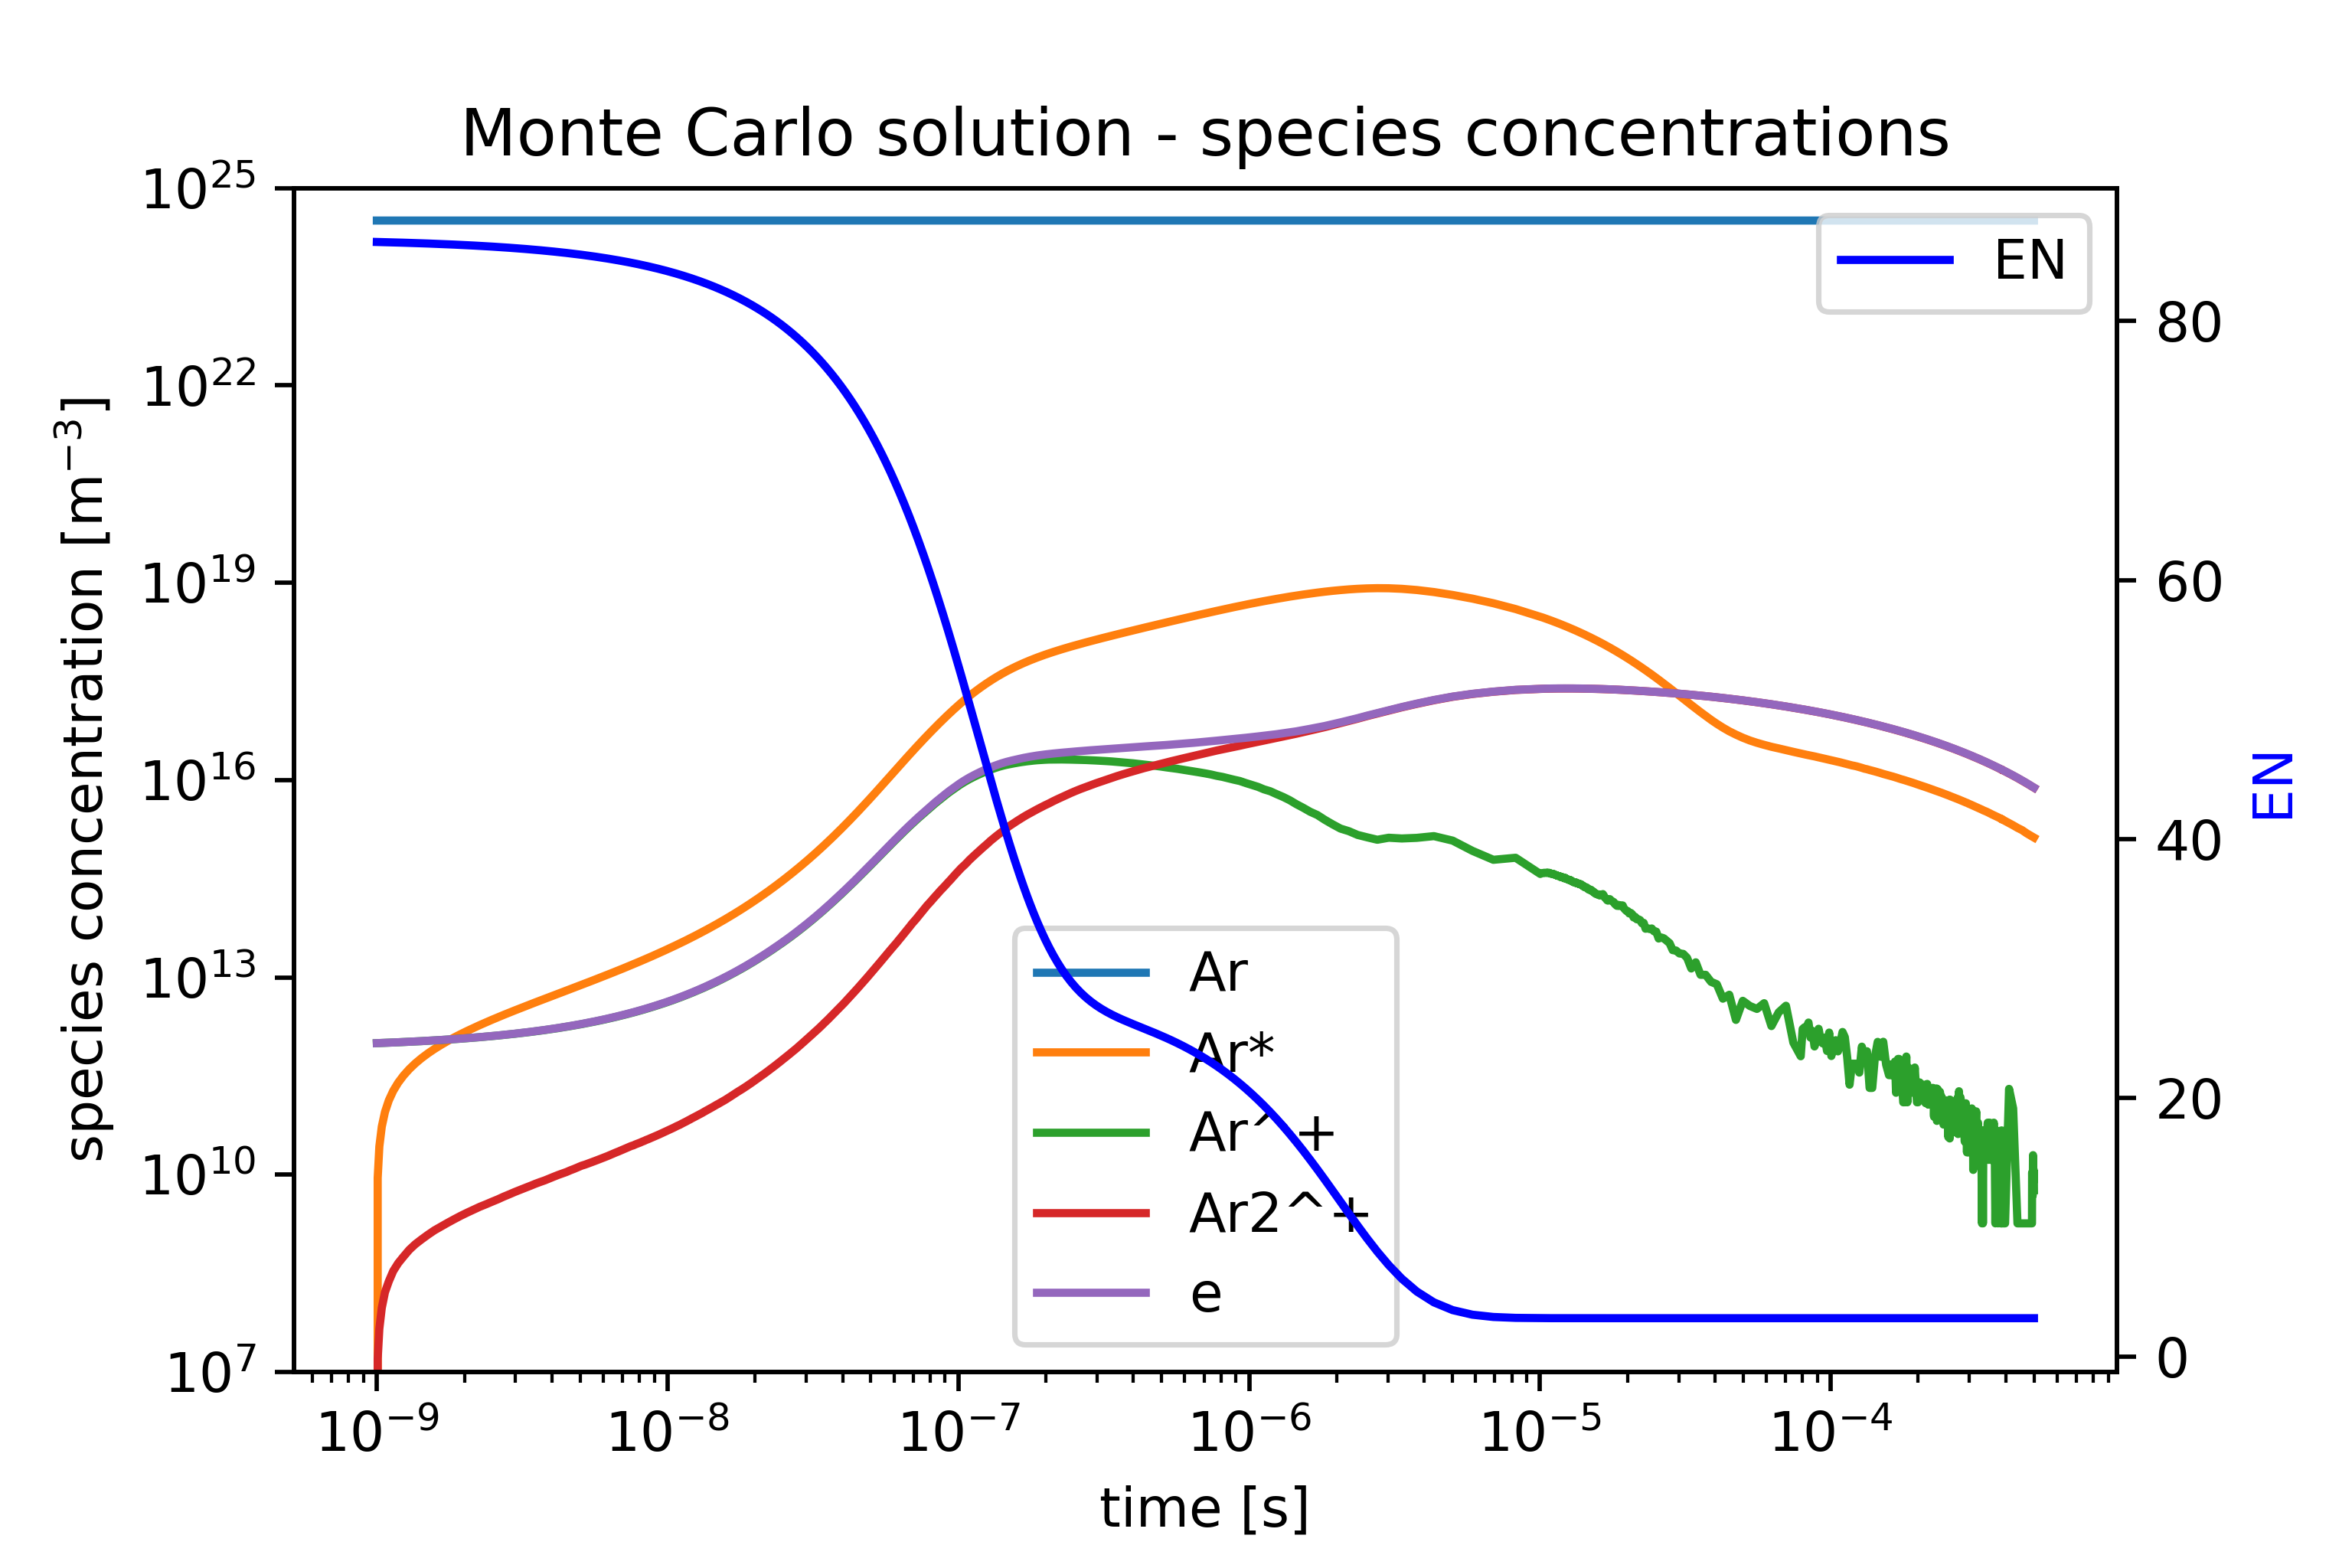
\includegraphics[width=\textwidth]{grafy/MicroCathodeImprovedMC.png}
    \caption{Micro cathode -- Monte Carlo solution for specie concentrations}
    \label{fig:MicroCathodeImprovedMC}
\end{figure}


In figure \ref{fig:MicroCathodeImprovedMCLosses} we examine the diffusion losses as computed during the simulation. Here, we observe noticeable discrepancies between the stochastic and the deterministic solution. Due to relatively rare concentrations of the species representing diffusion losses, executing the reactions in bulk makes the random fluctuations very visible. Later, when the concentrations grow, we see a perfect correspondence with the figure \ref{fig:MicroCathodeImprovedDeterministicLosses}.

\begin{figure} 
    \centering
    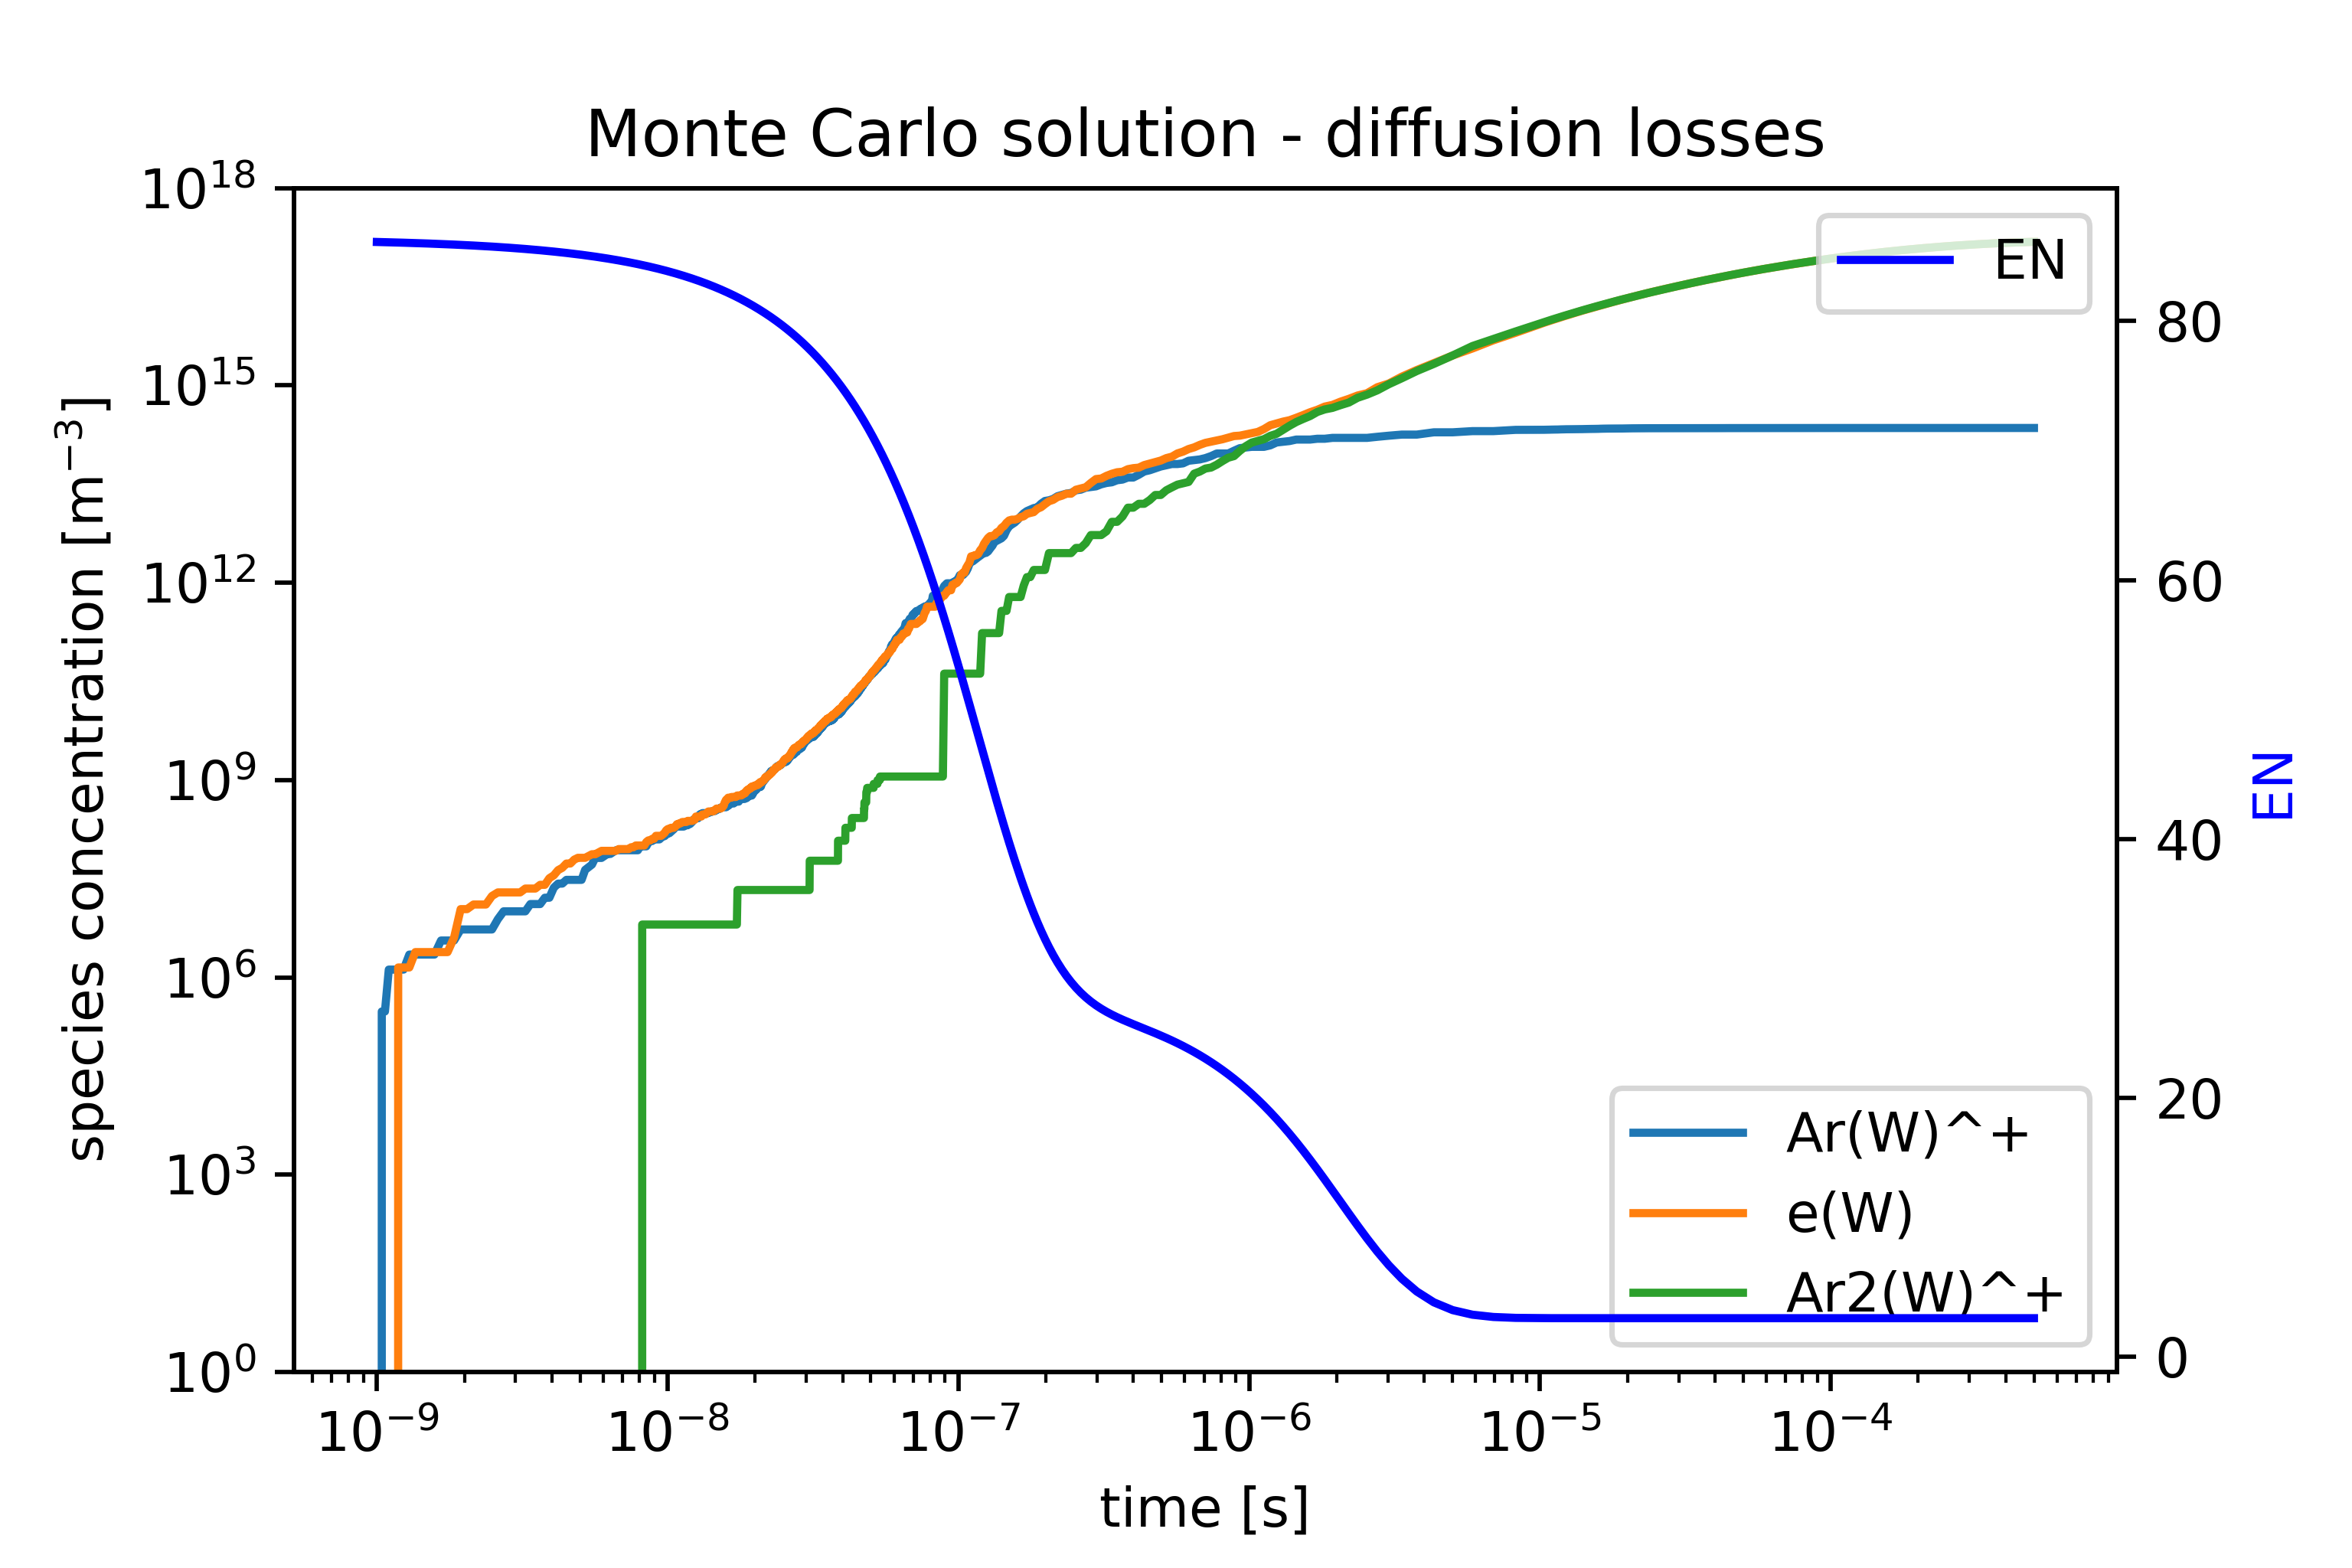
\includegraphics[width=\textwidth]{grafy/MicroCathodeImprovedMCLosses.png}
    \caption{Micro cathode -- Monte Carlo solution for diffusion losses}
    \label{fig:MicroCathodeImprovedMCLosses}
\end{figure}